\documentclass[xcolor=dvipsnames,notes]{beamer}
\usecolortheme[named=Brown]{structure}
\usetheme{default}
\setbeamertemplate{navigation symbols}{} 
\usepackage{tikz}
\usetikzlibrary{arrows,decorations.pathmorphing,backgrounds,positioning,fit}
\usetikzlibrary{datavisualization.formats.functions}
\usetikzlibrary{shapes}
\include{macro}
\usepackage{epsfig}
\usepackage{natbib}
\usepackage{graphicx}
\usepackage{multimedia}
\begin{document}
%\setbeamercolor{titlelike}{fg=gray,bg=white}
%\setbeamercolor{itemize item}{fg=gray,bg=white}
%\setbeamercolor{enumerate item}{fg=gray,bg=white}
%\setbeamercolor{block title}{fg=black,bg=white}
%==============================================
\title{TPG4190 Seismic data acquisition and processing \\
               Lecture 3: The CMP method}
\author{B. Arntsen}
\institute[NTNU]{
  NTNU\\
  Department of Geoscience and petroleum \\
  \texttt{borge.arntsen@ntnu.no}
}
\date{Trondheim fall 2021}
\begin{frame}
 \titlepage
\end{frame}
%==============================================
\begin{frame}{Overview}
%==============================================
\begin{itemize}
  \item Seismic data acquisition
   \item CMP method 2D
   \item CMP method 3D
   \item NMO and stack
   \item Wide azimuth
  \end{itemize}
\end{frame}
%-------------------------------------------------
\begin{frame}{Seismic marine data acquisition}
%-------------------------------------------------
%
\begin{figure}
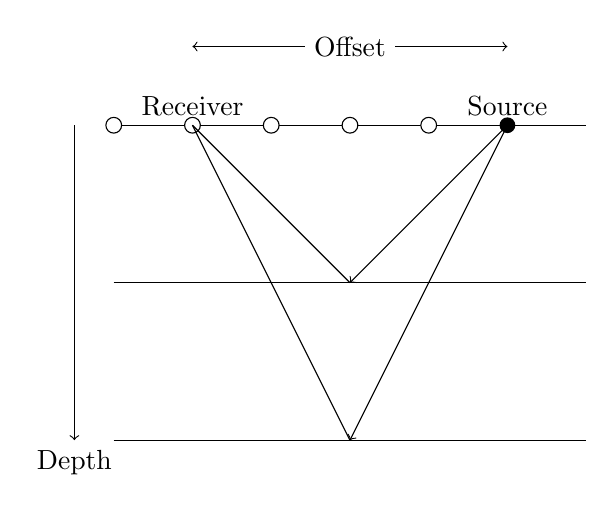
\begin{tikzpicture}
  \draw[->] (-0.5,4.0) -- (-0.5,0.0) node[below]{Depth} ;
  \draw[<->] (1.0,5.0) -- node[fill=white]{Offset} (5.0,5.0); 
  \draw (0.0,0.0) -- (6.0,0.0) ;
  \draw (0.0,2.0) -- (6.0,2.0) ;
  \draw (0.0,4.0) -- (6.0,4.0) ;
  \fill (5.0,4.0) node[above]{Source} circle (0.1) ;
  \fill[white] (0.0,4.0) circle (0.1) ;
  \draw (0.0,4.0) circle (0.1) ;
  \fill[white](1.0,4.0) circle (0.1) ;
  \draw (1.0,4.0) node[above]{Receiver}circle (0.1) ;
  \fill[white] (2.0,4.0) circle (0.1) ;
  \draw (2.0,4.0) circle (0.1) ;
  \fill[white] (3.0,4.0) circle (0.1) ;
  \draw (3.0,4.0) circle (0.1) ;
  \fill[white] (4.0,4.0) circle (0.1) ;
  \draw (4.0,4.0) circle (0.1) ;
  \draw[->] (5.0,4.0) -- (3.0,0.0) ;
  \draw (3.0,0.0) -- (1.0,4.0) ;
  \draw[->] (5.0,4.0) -- (3.0,2.0) ;
  \draw (3.0,2.0) -- (1.0,4.0) ;
\end{tikzpicture}
\label{fig:geom}
\end{figure}
\end{frame}
%
%-----------------------------------------
\begin{frame}{Schematic shot record}
%-----------------------------------------
%
\begin{figure}
  \includegraphics[width=0.8\textwidth]{Fig/schemshot.pdf}
  \caption{Schematic shot}
  \label{fig:shot}
\end{figure}
%
\end{frame}
%----------------------------------------------
\begin{frame}{Real shot record}
%----------------------------------------------
\begin{figure}
  \includegraphics[width=0.8\textwidth]{Fig/shotgath.pdf}
  \caption{Real shot}
  \label{fig:shotgath}
\end{figure}
%
%
\end{frame}
%-----------------------------------------
\begin{frame}{The cmp method}
%-----------------------------------------
%
\begin{figure}
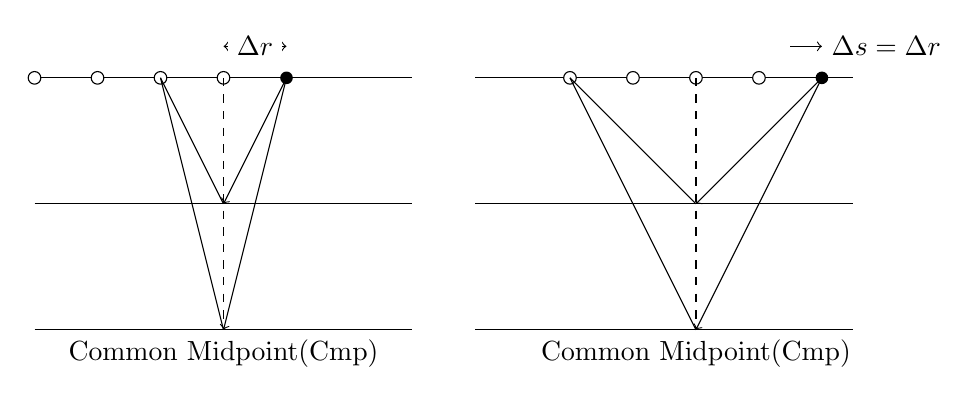
\begin{tikzpicture}[scale=0.8]
  \draw[<->] (3.0,4.5) -- node[fill=white]{$\Delta r$}(4.0,4.5); % Draw Delta r 
  \draw (0.0,0.0) -- (6.0,0.0) ;     %Draw Bottom reflector left display
  \draw (0.0,2.0) -- (6.0,2.0) ;     %Draw Middle reflector left display
  \draw (0.0,4.0) -- (6.0,4.0) ;     %Draw Surface left display
  \fill (4.0,4.0) circle (0.1) ;     %Draw source left display

  %Draw receivers on left display 

  \fill[white] (0.0,4.0) circle (0.1) ; 
  \draw (0.0,4.0) circle (0.1) ;
  \fill[white] (1.0,4.0) circle (0.1) ;
  \draw (1.0,4.0) circle (0.1) ;
  \fill[white] (2.0,4.0) circle (0.1) ;
  \draw (2.0,4.0) circle (0.1) ;
  \fill[white] (3.0,4.0) circle (0.1) ;
  \draw (3.0,4.0) circle (0.1) ;
 
  % Draw dashed vertical line and cmp text below bottom reflector left display
  \draw[dashed] (3.0,4.0) -- (3.0,0.0) node[below]{Common Midpoint(Cmp)} ;

  %Draw raypaths to bottom layer left display
  \draw[->] (4.0,4.0) -- (3.0,0.0) ; 
  \draw (3.0,0.0) -- (2.0,4.0) ;     

  %Draw raypaths to middle layer left display
  \draw[->] (4.0,4.0) -- (3.0,2.0) ;
  \draw (3.0,2.0) -- (2.0,4.0) ;

  \draw (7.0,0.0) -- (13.0,0.0) ; Draw bottom reflector right display
  \draw (7.0,2.0) -- (13.0,2.0) ; Draw middle reflector right display
  \draw (7.0,4.0) -- (13.0,4.0) ; Draw surface right display

  % Draw Delta s headline
  \fill (12.5,4.0) circle (0.1) ;
  \draw[->] (12.0,4.5) -- (12.5,4.5) node[right]{$\Delta s=\Delta r$};

  %Draw receivers on right display 
  \fill[white] (8.5,4.0)  circle (0.1) ;
  \draw (8.5,4.0)  circle (0.1) ;
  \fill[white] (9.5,4.0)  circle (0.1) ;
  \draw (9.5,4.0)  circle (0.1) ;
  \fill[white] (10.5,4.0) circle (0.1) ;
  \draw (10.5,4.0) circle (0.1) ;
  \fill[white] (11.5,4.0) circle (0.1) ;
  \draw (11.5,4.0) circle (0.1) ;

  %Draw raypaths to bottom layer
  \draw[->] (12.5,4.0) -- (10.5,0.0) ;
  \draw (10.5,0.0) -- (8.5,4.0) ;

  %Draw raypaths to middle layer
  \draw[->] (12.5,4.0) -- (10.5,2.0) ;
  \draw (10.5,2.0) -- (8.5,4.0) ;

  % Draw dashed vertical line and cmp text below bottom reflector left display
  \draw[dashed] (10.5,4.0) -- (10.5,0.0)node[below]{Common Midpoint(Cmp)} ;

\end{tikzpicture}
\label{fig:shotsgeom}
\end{figure}
%
\end{frame}
%--------------------------------------------
\begin{frame}{Common midpoint (cmp) gather}
%--------------------------------------------
\begin{figure}
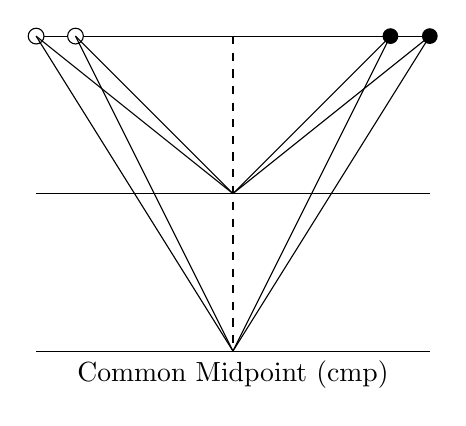
\begin{tikzpicture}
  \draw (0.0,0.0) -- (5.0,0.0) ;
  \draw (0.0,2.0) -- (5.0,2.0) ;
  \draw (0.0,4.0) -- (5.0,4.0) ;
  \fill[white] (0.0,4.0) circle (0.1) ;
  \draw (0.0,4.0) circle (0.1) ;
  \fill (5.0,4.0) circle (0.1) ;
  \fill[white] (0.5,4.0) circle (0.1) ;
  \draw (0.5,4.0) circle (0.1) ;
  \fill (4.5,4.0) circle (0.1) ;
  \draw[dashed] (2.5,4.0) -- (2.5,0.0)node[below]{Common Midpoint (cmp)} ;
  \draw (5.0,4.0) -- (2.5,2.0) ;
  \draw (2.5,2.0) -- (0.0,4.0) ;
  \draw (4.5,4.0) -- (2.5,2.0) ;
  \draw (2.5,2.0) -- (0.5,4.0) ;

  \draw (5.0,4.0) -- (2.5,0.0) ;
  \draw (2.5,0.0) -- (0.0,4.0) ;
  \draw (4.5,4.0) -- (2.5,0.0) ;
  \draw (2.5,0.0) -- (0.5,4.0) ;
\end{tikzpicture}
\label{fig:1-cmp}
\end{figure}
\end{frame}
%
%--------------------------------------------
\begin{frame}{Midpoint and Offset Coordinates}
%--------------------------------------------
\begin{eqnarray}
x_m & = & \frac{s+r}{2} ,\\
h   & = &  \frac{s-r}{2},
\label{eq:cmpcoord}
\end{eqnarray}
\begin{itemize}
  \item $x_m$: Midpoint coordinate
  \item $h$: Offset
  \item $s$: Source coordinate
  \item $r$: Receiver coordinate
\end{itemize}
\end{frame}
%----------------------------------------------
\begin{frame}{Midpoint and Offset Coordinates}
%----------------------------------------------
Assume that we change the source and
receiver coordinates a small amount $\delta s$ and $\delta r$.
The corresponding change in $x_m$ and $h$ are:
\begin{eqnarray}
\delta x_m & = & \frac{1}{2}\left(\delta s + \delta r\right) ,
                                              \label{eq:deltasrA}\\
\delta h   & = &  \frac{1}{2}\left(\delta s - \delta r\right).
                                              \label{eq:deltasrB}
\label{eq:deltasr}
\end{eqnarray}
If we consider a single cmp then $\delta x_m=0$
\begin{eqnarray}
0 & = & \frac{1}{2}\left(\delta s + \delta r\right) ,\\
\label{eq:deltasr2}
\end{eqnarray}
which implies
\begin{eqnarray}
\delta s = -\delta r
\label{eq:deltasr3}
\end{eqnarray}
\end{frame}
%----------------------------------------------
\begin{frame}{Midpoint and Offset Coordinates}
%----------------------------------------------
Inserting equation \eqref{eq:deltasr3} into
equation \eqref{eq:deltasrB} I get
\begin{eqnarray}
\delta h = \delta s = \delta r
\label{eq:deltasr4}
\end{eqnarray}
We can now deduce the number of traces in each cmp, or the fold.
The largest (half offset) is equal to 
\begin{eqnarray}
h_{max}=\frac{N_r}{2} \Delta r
\end{eqnarray}
where
\begin{itemize}
\item $\Delta r$ : Distance between receiver groups
\item $N_r$ : Number of receivers
\end{itemize}
The fold $N_f$ is then
\begin{eqnarray}
 N_f = \frac{h_{max}}{\delta h} = \frac{N_r}{2} \frac{\Delta r}{\delta s}
\end{eqnarray}
\end{frame}
%----------------------------------------------
\begin{frame}{Midpoint and Offset Coordinates}
%----------------------------------------------
It remains to specify $\delta s$. 
The simplest assumption we can make is that $\delta s = \Delta s$,
where $\Delta s$ is the distance between shots.
The final expression for the fold $N_f$ is then
\begin{eqnarray}
 N_f = \frac{h_{max}}{\delta h} = \frac{N_r}{2} \frac{\Delta r}{\Delta s}
\end{eqnarray}
We can also figure out the distance between consecutive cmp's
if we assume that the change in $\delta r$ is equal to the receiver group spacing $\Delta r$
and that $\Delta r < \Delta s$ and use equation \eqref{eq:deltasrA}
\begin{eqnarray}
\delta x_m & = & \frac{1}{2}\Delta r
\label{eq:deltacmp}
\end{eqnarray}
\end{frame}
%-------------------------------------------------
\begin{frame}{Midpoint and Offset Coordinates}
%-------------------------------------------------
Example:\\
\begin{itemize}
  \item No of receivers: 10 
  \item No of shots: 5
  \item $\Delta r = \Delta s = 25.0$m
  \item $\Delta x_m=$12.5m, $N_f$ = 10/2 = 5
\end{itemize}

\begin{figure}
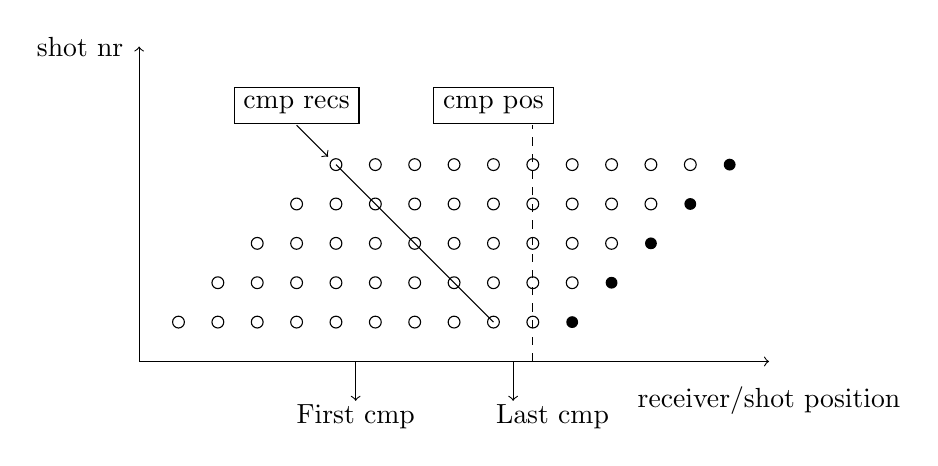
\begin{tikzpicture}
    \pgfmathsetmacro {\lx}{8}  %Length of x-axis
    \pgfmathsetmacro {\ly}{4}  %Length of y-axis
    \draw[->] (0,0) -- (\lx,0);% Draw x-axis
    \draw[->] (0,0) -- (0,\ly);% Draw y-axis
    \node at (-0.75,\ly) {shot nr};                 % Y axis label
    \node at (\lx,-0.5) {receiver/shot position};   % X axis label
    
    \pgfmathsetmacro {\ns }{5}  %No of shots
    \pgfmathsetmacro {\nns }{4} %No of shots-1
    \pgfmathsetmacro {\nr }{10} %No of receivers
    \pgfmathsetmacro {\nnr}{9}  %No of receivers-1
    \pgfmathsetmacro {\dr}{0.5} %Receiver spacing

    %Loop for drawing receiver positions and shot positions
    \foreach \j in {0,...,\nns} {
        \pgfmathsetmacro {\y}{ \j*0.5+0.5}        %receiver y-position
        \pgfmathsetmacro {\s}{0.5*\nr+0.5*\j+0.5} %shot position
        \fill[black] (\s,\y) circle (0.075);        %Draw sources position
        \foreach \i in {0,...,\nnr} {
            \pgfmathsetmacro {\x}{ \i*0.5+0.5*\j+0.5} %Receiver x-position
            \fill[white] (\x,\y) circle (0.075) ;     %Draw receivers
            \draw        (\x,\y) circle (0.075) ;     %Draw receivers
        }
    }

    %
    % Marking example cmp gather
    %
    \pgfmathsetmacro {\cmpxl}{4*\dr+0.5} %x-coordinate last rec cmp gather
    \pgfmathsetmacro {\cmpyl}{4*\dr+0.5} %y-coordinate last rec cmp gather
    \pgfmathsetmacro {\cmpxf}{5*\dr+2.0} %y-coordinate first rec cmp gather
    \pgfmathsetmacro {\cmpyf}{0.5}       %y-coordinate first rec cmp gather
    \draw (\cmpxf,\cmpyf) -- (\cmpxl,\cmpyl); %Mark cmp gather
    %Create receiver text box
    \node[draw] at (\cmpxl-0.5,\cmpyl+0.75) {cmp recs} ;
    %Draw arrow pointing from text box to receeivers
    \draw[->] (\cmpxl-0.5,\cmpyl+0.5) -- (\cmpxl-0.1,\cmpyl+0.1);
    \draw[dashed] (5,0) -- (5,3) ;  %Mark corresponding cmp position
    %Create position text box
    \node[draw] at (3.5+1,3+0.25) {cmp pos};

    %
    % Draw annotation for first and last cmp position
    %
    \pgfmathsetmacro {\cmpxf}{4*\dr+0.5+0.25}
    \draw[->] (\cmpxf,0) -- (\cmpxf,-0.5) ;
    \node at (\cmpxf,-0.7) {First cmp }; 
    \pgfmathsetmacro {\cmpxl}{8*\dr+0.5+0.25}
    \draw[->] (\cmpxl,0) -- (\cmpxl,-0.5) ;
    \node at (\cmpxl+0.5,-0.7) {Last cmp }; 
\end{tikzpicture}
\label{fig:nmop}
\end{figure}
\end{frame}
%-------------------------------------------------
\begin{frame}{Aqcuisition geometry 3D}
%-------------------------------------------------
\begin{figure}
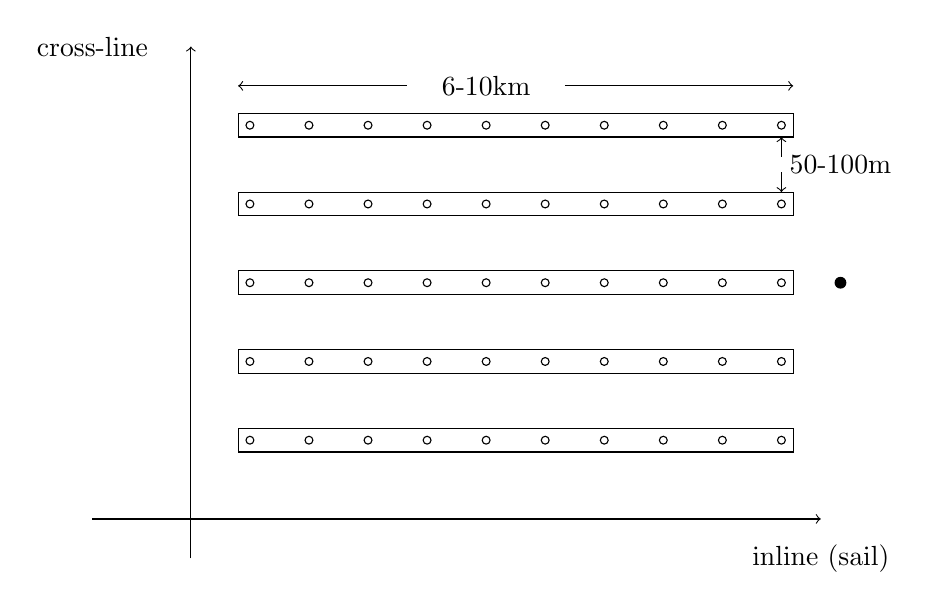
\begin{tikzpicture}
    \pgfmathsetmacro {\lx}{8}  %Length of x-axis
    \pgfmathsetmacro {\ly}{6}  %Length of y-axis
    \draw[->] (-1.25,0) -- (\lx,0);        % Draw x-axis
    \draw[->] (0,-0.5) -- (0,\ly);         % Draw y-axis
    \node at (-1.25,\ly) {cross-line};     % Y axis label
    \node at (\lx,-0.5) {inline (sail)};   % X axis label
    
    \pgfmathsetmacro {\ns }{5}   %No of shots
    \pgfmathsetmacro {\nr }{10}  %No of receivers
    \pgfmathsetmacro {\dr}{0.75} %Receiver spacing
    \pgfmathsetmacro {\dl}{1.0}  %Shot line separation

    %Loop for drawing receiver positions and shot positions
    \foreach \j in {1,...,\ns} {
        \pgfmathsetmacro {\y}{\j*\dl}        %receiver y-position
        \foreach \i in {1,...,\nr} {
            \pgfmathsetmacro {\x}{ \i*\dr}            %Receiver x-position
            \fill[white] (\x,\y) circle (0.050) ;     %Draw receivers
            \draw (\x,\y) circle (0.050) ;            %Draw receivers
            %Draw cables
            \draw (\dr-0.15,\y-0.15) rectangle (\nr*\dr+0.15,\y+0.15);
        }
    }
    \pgfmathsetmacro {\s}{\dr*\nr+\dr}   %shot position
    \pgfmathsetmacro {\y}{3*\dl}         %shot y-position
    \fill[black] (\s,\y) circle (0.075);   %Draw source position

    %Draw cable length annotation
    \draw[<-]  (\dr-0.15,\dl*\ns+0.5) -- (\nr*\dr/2-1.0,\dl*\ns+0.5);
    \node at   (\nr*\dr/2,\dl*\ns+0.5) {6-10km};
    \draw[->]  (\nr*\dr/2+1.0,\dl*\ns+0.5) -- (\nr*\dr+0.15,\dl*\ns+0.5);

    %Draw streamer separation annotation
    \draw[<-]  (\nr*\dr,\dl*\ns-0.15)-- (\nr*\dr,\dl*\ns-0.15-\dl*0.25);
    \node at   (\nr*\dr+\dr,\dl*\ns-0.15-\dl*0.25-0.1) {50-100m};
    \draw[->]  (\nr*\dr,\dl*\ns-0.15-\dl*0.25-0.2) -- 
               (\nr*\dr,\dl*\ns-0.15-\dl*0.25-0.45);
\end{tikzpicture}
\label{fig:nmop}
\end{figure}
\end{frame}
%----------------------------------------------------------------
\begin{frame}{3D Seismic marine data acquisition single source}
%----------------------------------------------------------------
%
\begin{figure}
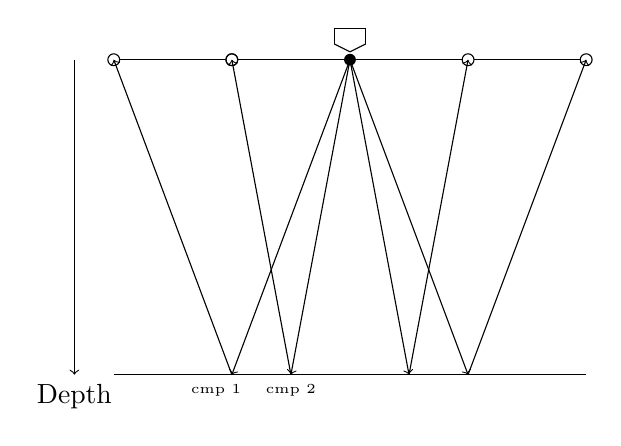
\begin{tikzpicture}
  \pgfmathsetmacro {\nl}{4}   %no of cables
  \pgfmathsetmacro {\dl}{1.5}   %cable separation
  \pgfmathsetmacro {\xl}{\dl*\nl} %cross-line coordinate
  \pgfmathsetmacro {\sx}{\dl*2.0} %Source cross line coordinate
  \pgfmathsetmacro {\rd}{0.075} %Receiver diameter
  
  \draw[->] (-0.5,4.0) -- (-0.5,0.0) node[below]{Depth} ; %Draw vertical axis
  \draw (0.0,0.0) -- (\xl,0.0) ; %Interface 2
  %\draw (0.0,2.0) -- (\xl,2.0) ; %Interface 1

  %Draw receivers and source
  \draw (0.0,4.0) -- (\xl,4.0) ; %Receiver line
  \fill[white] (0.0,4.0) circle (\rd) ;     %Receiver no 1
  \draw (0.0,4.0) circle (\rd) ;            %Receiver 1 outline
  \fill[white](\dl,4.0) circle (\rd) ;      %Receiver no 2
  \draw(\dl,4.0) circle (\rd) ;             %Receiver no 2
  \draw (\dl,4.0) circle (\rd) ;            %Receiver 2 outline fill
  \fill[black] (\sx,4.0) circle (\rd) ; %Source

  %Draw a boat (!)
  \pgfmathsetmacro {\dd}{0.1} %Depth of keel
  \pgfmathsetmacro {\bw}{0.4} %Boat width
  \pgfmathsetmacro {\bh}{0.2} %Boat hight (above keel)
  \pgfmathsetmacro {\bk}{0.1} %Boat keel hight 
  \draw (\sx,4.0+\dd) -- (\sx-\bw/2,4.0+\bk+\dd) ;
  \draw (\sx,4.0+\dd) -- (\sx+\bw/2,4.0+\bk+\dd) ;
  \draw (\sx+\bw/2,4.0+\bk+\dd) -- (\sx+\bw/2,4.0+\bk+\bh+\dd);
  \draw (\sx-\bw/2,4.0+\bk+\dd) -- (\sx-\bw/2,4.0+\bk+\bh+\dd);
  \draw (\sx-\bw/2,4.0+\bk+\bh+\dd) -- (\sx+\bw/2,4.0+\bk+\bh+\dd);' 


  \fill[white] (3*\dl,4.0) circle (\rd) ;   %Receiver 3
  \draw (3*\dl,4.0) circle (\rd) ;          %Receiver 3 outline
  \fill[white] (4.0*\dl,4.0) circle (\rd) ; %Receiver no 4
  \draw (4.0*\dl,4.0) circle (\rd) ;        %Receiver no 4 outline

  %Draw ray paths to the left of source
  \draw[->] (\sx,4.0) -- (\sx-\dl/2,0.0) ;  
  \draw[->] (\sx-\dl/2,0.0) -- (\sx-\dl,4.0) ;
  \node[below] at (\sx-\dl/2,0.0) {\tiny cmp 2};
  \draw[->] (\sx,4.0) -- (\sx-\dl,0.0) ;
  \draw[->] (\sx-\dl,0.0) -- (\sx-2*\dl,4.0) ;

  %Draw ray paths to the right of source
  \draw[->] (\sx,4.0) -- (\sx+\dl/2,0.0) ;  
  \draw[->] (\sx+\dl/2,0.0) -- (\sx+\dl,4.0) ;
  \node[below] at (\sx-\dl-0.2,0.0) {\tiny cmp 1};
  \draw[->] (\sx,4.0) -- (\sx+\dl,0.0) ;
  \draw[->] (\sx+\dl,0.0) -- (\sx+2*\dl,4.0) ;


\end{tikzpicture}
\label{fig:geom}
\end{figure}
\end{frame}
%------------------------------------------------------------------
\begin{frame}{3D Seismic marine data acquisition flip-flop (left)}
%------------------------------------------------------------------
%
\begin{figure}
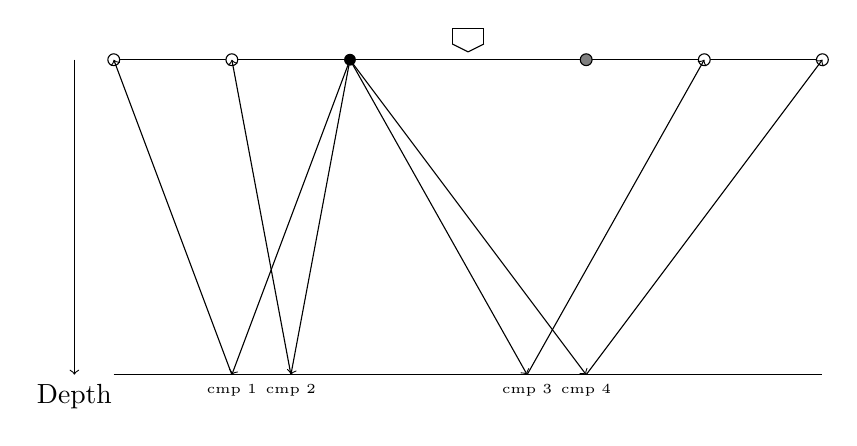
\begin{tikzpicture}
  \pgfmathsetmacro {\nl}{6}   %no of cables
  \pgfmathsetmacro {\dl}{1.5}   %cable separation
  \pgfmathsetmacro {\xl}{\dl*\nl} %cross-line coordinate
  \pgfmathsetmacro {\sx}{\dl*3.0} %Source cross line coordinate
  \pgfmathsetmacro {\sxa}{\sx-\dl} %Source cross line coordinate
  \pgfmathsetmacro {\sxb}{\sx+\dl} %Source cross line coordinate
  \pgfmathsetmacro {\rd}{0.075} %Receiver diameter
  
  \draw[->] (-0.5,4.0) -- (-0.5,0.0) node[below]{Depth} ; %Draw vertical axis
  \draw (0.0,0.0) -- (\xl,0.0) ; %Interface 2
  %\draw (0.0,2.0) -- (\xl,2.0) ; %Interface 1

  %Draw receivers and source
  \draw (0.0,4.0) -- (\xl,4.0) ; %Receiver line
  \fill[white] (0.0,4.0) circle (\rd) ;     %Receiver no 1
  \draw (0.0,4.0) circle (\rd) ;            %Receiver 1 outline
  \fill[white](\dl,4.0) circle (\rd) ;      %Receiver no 2
  \draw (\dl,4.0) circle (\rd) ;            %Receiver 2 outline fill
  \fill[black] (\sxa,4.0) circle (\rd) ;    %Source left
  \fill[gray] (\sxb,4.0) circle (\rd) ;    %Source right
  \draw (\sxb,4.0) circle (\rd) ;           %Source right outline

  %Draw a boat (!)
  \pgfmathsetmacro {\dd}{0.1} %Depth of keel
  \pgfmathsetmacro {\bw}{0.4} %Boat width
  \pgfmathsetmacro {\bh}{0.2} %Boat hight (above keel)
  \pgfmathsetmacro {\bk}{0.1} %Boat keel hight 
  \draw (\sx,4.0+\dd) -- (\sx-\bw/2,4.0+\bk+\dd) ;
  \draw (\sx,4.0+\dd) -- (\sx+\bw/2,4.0+\bk+\dd) ;
  \draw (\sx+\bw/2,4.0+\bk+\dd) -- (\sx+\bw/2,4.0+\bk+\bh+\dd);
  \draw (\sx-\bw/2,4.0+\bk+\dd) -- (\sx-\bw/2,4.0+\bk+\bh+\dd);
  \draw (\sx-\bw/2,4.0+\bk+\bh+\dd) -- (\sx+\bw/2,4.0+\bk+\bh+\dd);' 


  \fill[white] (\sx+2*\dl,4.0) circle (\rd) ; %Receiver 3
  \draw (\sx+2*\dl,4.0) circle (\rd) ;        %Receiver 3 outline
  \fill[white] (\sx+3*\dl,4.0) circle (\rd) ; %Receiver no 4
  \draw (\sx+3*\dl,4.0) circle (\rd) ;        %Receiver no 4 outline
  \pgfmathsetmacro {\dha}{\sxa-\dl}           %Offset left source - rec2
  \pgfmathsetmacro {\dhaa}{\sxa}                 %Offset left source - rec1
  \pgfmathsetmacro {\dhb}{\sx+2*\dl-\sxa}     %cable separation
  \pgfmathsetmacro {\dhbb}{\sx+3*\dl-\sxa}    %cable separation

  %Draw ray paths to the left of source
  \draw[->] (\sxa,4.0) -- (\sxa-\dha/2,0.0) ;  
  \draw[->] (\sxa-\dha/2,0.0) -- (\sxa-\dha,4.0) ;
  \node[below] at (\sxa-\dha/2,0.0) {\tiny cmp 2};
  \draw[->] (\sxa,4.0) -- (\sxa-\dhaa/2,0.0) ;
  \draw[->] (\sxa-\dhaa/2.0,0.0) -- (\sxa-\dhaa,4.0) ;
  \node[below] at (\sxa-\dhaa/2,0.0) {\tiny cmp 1};

  %Draw ray paths to the right of source
  \draw[->] (\sxa,4.0) -- (\sxa+\dhb/2,0.0) ;  
  \draw[->] (\sxa+\dhb/2,0.0) -- (\sxa+\dhb,4.0) ;
  \node[below] at (\sxa+\dhb/2,0.0) {\tiny cmp 3};
  \draw[->] (\sxa,4.0) -- (\sxa+\dhbb/2,0.0) ;  
  \draw[->] (\sxa+\dhbb/2,0.0) -- (\sxa+\dhbb,4.0) ;
  \node[below] at (\sxa+\dhbb/2,0.0) {\tiny cmp 4};
\end{tikzpicture}
\label{fig:geom}
\end{figure}
\end{frame}
%--------------------------------------------------------------------
\begin{frame}{3D Seismic marine data acquisition flip-flop (right)}
%--------------------------------------------------------------------
%
\begin{figure}
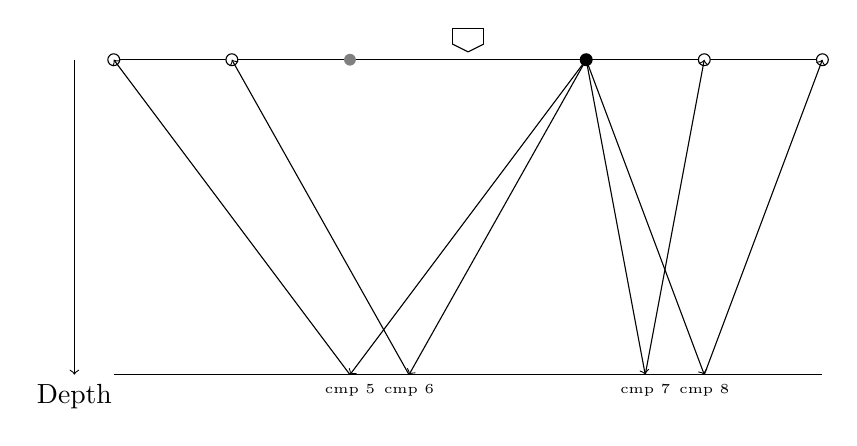
\begin{tikzpicture}
  \pgfmathsetmacro {\nl}{6}   %no of cables
  \pgfmathsetmacro {\dl}{1.5}   %cable separation
  \pgfmathsetmacro {\xl}{\dl*\nl} %cross-line coordinate
  \pgfmathsetmacro {\sx}{\dl*3.0} %Source cross line coordinate
  \pgfmathsetmacro {\sxa}{\sx+\dl} %Source cross line coordinate
  \pgfmathsetmacro {\sxb}{\sx-\dl} %Source cross line coordinate
  \pgfmathsetmacro {\rd}{0.075} %Receiver diameter
  
  \draw[->] (-0.5,4.0) -- (-0.5,0.0) node[below]{Depth} ; %Draw vertical axis
  \draw (0.0,0.0) -- (\xl,0.0) ; %Interface 2
  %\draw (0.0,2.0) -- (\xl,2.0) ; %Interface 1

  %Draw receivers and source
  \draw (0.0,4.0) -- (\xl,4.0) ; %Receiver line
  \fill[white] (0.0,4.0) circle (\rd) ;     %Receiver no 1
  \draw (0.0,4.0) circle (\rd) ;            %Receiver 1 outline
  \fill[white](\dl,4.0) circle (\rd) ;      %Receiver no 2
  \draw (\dl,4.0) circle (\rd) ;            %Receiver 2 outline fill
  \fill[black] (\sxa,4.0) circle (\rd) ; %Source
  \draw (\sxa,4.0) circle (\rd) ;       
  \fill[gray] (\sxb,4.0) circle (\rd) ; %Source

  %Draw a boat (!)
  \pgfmathsetmacro {\dd}{0.1} %Depth of keel
  \pgfmathsetmacro {\bw}{0.4} %Boat width
  \pgfmathsetmacro {\bh}{0.2} %Boat hight (above keel)
  \pgfmathsetmacro {\bk}{0.1} %Boat keel hight 
  \draw (\sx,4.0+\dd) -- (\sx-\bw/2,4.0+\bk+\dd) ;
  \draw (\sx,4.0+\dd) -- (\sx+\bw/2,4.0+\bk+\dd) ;
  \draw (\sx+\bw/2,4.0+\bk+\dd) -- (\sx+\bw/2,4.0+\bk+\bh+\dd);
  \draw (\sx-\bw/2,4.0+\bk+\dd) -- (\sx-\bw/2,4.0+\bk+\bh+\dd);
  \draw (\sx-\bw/2,4.0+\bk+\bh+\dd) -- (\sx+\bw/2,4.0+\bk+\bh+\dd);' 


  \fill[white] (\sx+2*\dl,4.0) circle (\rd) ;   %Receiver 3
  \draw (\sx+2*\dl,4.0) circle (\rd) ;          %Receiver 3 outline
  \fill[white] (\sx+3*\dl,4.0) circle (\rd) ; %Receiver no 4
  \draw (\sx+3*\dl,4.0) circle (\rd) ;        %Receiver no 4 outline
  \pgfmathsetmacro {\dha}{\sxa-\dl}   %cable separation
  \pgfmathsetmacro {\dhaa}{\sxa}   %cable separation
  \pgfmathsetmacro {\dhb}{\sx+2*\dl-\sxa}   %cable separation
  \pgfmathsetmacro {\dhbb}{\sx+3*\dl-\sxa}   %cable separation

  %Draw ray paths to the left of source
  \draw[->] (\sxa,4.0) -- (\sxa-\dha/2,0.0) ;  
  \draw[->] (\sxa-\dha/2,0.0) -- (\sxa-\dha,4.0) ;
  \node[below] at (\sxa-\dha/2,0.0) {\tiny cmp 6};
  \draw[->] (\sxa,4.0) -- (\sxa-\dhaa/2,0.0) ;
  \draw[->] (\sxa-\dhaa/2.0,0.0) -- (\sxa-\dhaa,4.0) ;
  \node[below] at (\sxa-\dhaa/2,0.0) {\tiny cmp 5};

  %Draw ray paths to the right of source
  \draw[->] (\sxa,4.0) -- (\sxa+\dhb/2,0.0) ;  
  \draw[->] (\sxa+\dhb/2,0.0) -- (\sxa+\dhb,4.0) ;
  \node[below] at (\sxa+\dhb/2,0.0) {\tiny cmp 7};
  \draw[->] (\sxa,4.0) -- (\sxa+\dhbb/2,0.0) ;  
  \draw[->] (\sxa+\dhbb/2,0.0) -- (\sxa+\dhbb,4.0) ;
  \node[below] at (\sxa+\dhbb/2,0.0) {\tiny cmp 8};
\end{tikzpicture}
\label{fig:geom}
\end{figure}
\end{frame}
%-------------------------------------------------
\begin{frame}{3D Binning}
%-------------------------------------------------
\begin{figure}
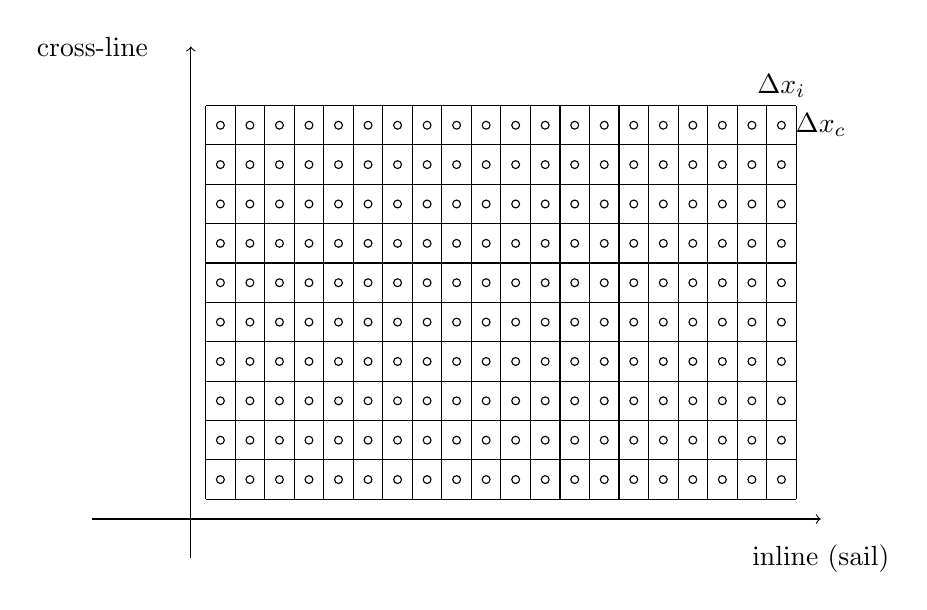
\begin{tikzpicture}
    \pgfmathsetmacro {\lx}{8}  %Length of x-axis
    \pgfmathsetmacro {\ly}{6}  %Length of y-axis
    \draw[->] (-1.25,0) -- (\lx,0);        % Draw x-axis
    \draw[->] (0,-0.5) -- (0,\ly);         % Draw y-axis
    \node at (-1.25,\ly) {cross-line};     % Y axis label
    \node at (\lx,-0.5) {inline (sail)};   % X axis label
    
    \pgfmathsetmacro {\ns }{10}   %No of cables
    \pgfmathsetmacro {\nr }{20}   %No of receivers
    \pgfmathsetmacro {\nnr }{21}  %No of receivers + 1
    \pgfmathsetmacro {\dr}{0.75/2}%Receiver spacing
    \pgfmathsetmacro {\dl}{0.5}   %Streamer separation

    %Loop for drawing receiver positions and shot positions
    \foreach \j in {1,...,\ns} {
        \pgfmathsetmacro {\y}{\j*\dl}        %receiver y-position
        \foreach \i in {1,...,\nr} {
            \pgfmathsetmacro {\x}{ \i*\dr}            %Receiver x-position
            \fill[white] (\x,\y) circle (0.050) ;     %Draw receivers
            \draw (\x,\y) circle (0.050) ;            %Draw receivers
                                                      
        }
    }

    %Loop for drawing bins (grid) in in-line dir:
    \foreach \j in {0,...,\ns} {
         \draw (\dr-0.5*\dr,\j*\dl+0.5*\dl) -- (\nr*\dr+0.5*\dr,\j*\dl+0.5*\dl);
    }
    %Loop for drawing bins (grid) in x-line dir:
    \foreach \j in {1,...,\nnr} {
         \draw (\j*\dr-0.5*\dr,0.5*\dl) -- (\j*\dr-0.5*\dr,\ns*\dl+0.5*\dl);
    }

   % In-line X-line sizes
    \node at (\nr*\dr,\ns*\dl+0.5) {$\Delta x_i$};
    \node at (\nr*\dr+0.5,\ns*\dl) {$\Delta x_c$};
\end{tikzpicture}
\label{fig:nmop}
\end{figure}
\end{frame}
%-----------------------------------------
\begin{frame}{NMO and Stack}
%-----------------------------------------
\begin{figure}
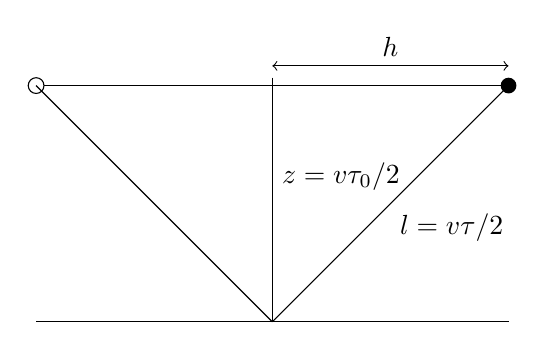
\begin{tikzpicture}
  \draw (0.0,1.0) -- (6.0,1.0) ;
  \draw (0.0,4.0) -- (6.0,4.0) ;
  \draw[<->](3.0,4.25) -- node[above]{$h$}(6.0,4.25) ;
  \fill[white] (0.0,4.0) circle (0.1) ;
  \draw (0.0,4.0) circle (0.1) ;
  \fill (6.0,4.0) circle (0.1) ;
  \draw (6.0,4.0) -- node[below right]{$l=v\tau/2$}(3.0,1.0) ;
  \draw (3.0,1.0) -- (0.0,4.0) ;
  \draw (3.0,4.1) -- node[above right]{$z=v\tau_0/2$}(3.0,1.0) ;
\end{tikzpicture}
\label{fig:nmop}
\end{figure}

The traveltime $\tau(h)$ is:
%
\begin{eqnarray}
l^2 = z^2+h^2 \nonumber\\
\end{eqnarray}
which gives by inserting $v\tau/2$ for $l$ and $v\tau_0/2$ for $z$
\begin{eqnarray}
\tau(h)=\sqrt{\tau^2_0+4h^2/v^2}.
\label{eq:nmo}
\end{eqnarray}
\end{frame}
%-----------------------------------------
\begin{frame}{NMO and Stack}
%-----------------------------------------
Nmo-correction:
%
\begin{eqnarray}
 \Delta \tau = \tau(h)-\tau_0,
\label{eq:dtnmo}
\end{eqnarray}
\end{frame}
%
%-----------------------------------------
\begin{frame}{Cmp}
%-----------------------------------------
\begin{figure}
  \includegraphics[width=0.8\textwidth]{Fig/synshot.pdf}
  \caption{}
  \label{fig:synshot}
\end{figure}
\end{frame}
%-----------------------------------------
\begin{frame}{Nmo}
%-----------------------------------------
\begin{figure}
  \includegraphics[width=0.8\textwidth]{Fig/syncmp.pdf}
  \caption{Synthetic cmp}
  \label{fig:syncmp}
\end{figure}
\end{frame}
%-----------------------------------------
\begin{frame}{Stack}
%-----------------------------------------
\begin{figure}
  \includegraphics[width=0.8\textwidth]{Fig/synstack.pdf}
  \caption{Synthetic stack}
  \label{fig:synstack}
\end{figure}
\end{frame}
%-----------------------------------------
\begin{frame}{NMO and Stack}
%-----------------------------------------
Average velocity $v_{rms}$ defined by
\begin{eqnarray}
 v^2_{rms}(t_0)=\frac{1}{t_0}\int^{t_0}_0 v^2(t)dt
\label{eq:rms}
\end{eqnarray}
$v(t)$ : Interval velocity.
The traveltime equation \eqref{eq:nmo} then becomes
\begin{eqnarray}
\tau(h)=\sqrt{t^2_0+4h^2/v^2_{rms}(t_0)}.
\label{eq:nmorms}
\end{eqnarray}
\end{frame}
%----------------------------------------------------
\begin{frame}{Real cmp}
%----------------------------------------------------
\begin{figure}
  \includegraphics[width=0.6\textwidth]{Fig/cmp.pdf}
  \caption{Real cmp}
  \label{fig:cmp}
\end{figure}
\end{frame}
%----------------------------------------------------
\begin{frame}{Real stack}
%----------------------------------------------------
\begin{figure}
  \includegraphics[width=0.8\textwidth]{Fig/stack.pdf}
  \caption{Real stack}
  \label{fig:stack}
\end{figure}
\end{frame}
%----------------------------------------------------
\begin{frame}{Wide azimuth}
%----------------------------------------------------
\begin{figure}
  \includegraphics[width=0.8\textwidth]{Fig/wats-7.eps}
  \caption{Real stack}
  \label{fig:wats2}
\end{figure}
\end{frame}
%----------------------------------------------------
\begin{frame}{Wide azimuth}
%----------------------------------------------------
\begin{figure}
  \includegraphics[width=0.8\textwidth]{Fig/wats.png}
  \caption{Real stack}
  \label{fig:wats1}
\end{figure}
\tiny Source:
https://www.pgs.com/publications/feature-stories/why-more-azimuths-is-a-good-thing/
\end{frame}
%-----------------------------------------
\begin{frame}{Velocity analysis}
%-----------------------------------------
%
  Estimate $v_{rms}$ from equation \eqref{eq:nmo}
\begin{enumerate}
  \item Make a guess of $v$ 
  \item Perform Nmo correction for all $t_0$ with using guess of $v$
  \item Make a stack trace
  \item Perform above steps for a range of guesses of $v$
  \item Plot all stack traces in a velocity spectrum
\end{enumerate}
\end{frame}
%-----------------------------------------
\begin{frame}{Velocity spectrum}
%-----------------------------------------
 \plot{synscn}{width=0.5\textwidth}{}
\end{frame}
%-----------------------------------------
\begin{frame}{Semblance}
%-----------------------------------------
Stack is usually replaced with semblance to
get better velocity spectra  
\begin{eqnarray}
S(t) = \frac{\int_0^{h_{max}} p^2(t,h)}{\int dt_0^T\, \int_0^{h_{max}} p^2(t,h)}
\end{eqnarray}
\begin{itemize}
 \item $p(t,h)$ : data 
 \item $h_{max}$: maximum offset. 
\end{itemize}
This equation can not be used directly.  Why?
\end{frame}
%
%-----------------------------------------
\begin{frame}{Semblance}
%-----------------------------------------
\begin{eqnarray}
S_k = \frac{\sum_{i=0}^{N_h} p^2_{k,i}}{\sum_{k=0}^{N_t} \sum_{i=0}^{N_h} p^2_{k,i}}
\end{eqnarray}
\begin{itemize}
 \item $S_k = S(t=k\Delta t), k=0,\ldots,N_t$ 
 \item $p_{k,i}=p(t=k\Delta t,h=i\Delta h), i=0,\ldots,N_h$. 
 \item $\Delta t$ time sampling interval, 
 \item $\Delta h$ distance between offsets \item $N_t$,$N_h$ :
No of time samples and No of  offsets
\end{itemize}
\end{frame}
%-----------------------------------------
\begin{frame}{Velocity analysis}
%-----------------------------------------
 \plot{synvel}{width=0.5\textwidth}{}
\end{frame}
%-----------------------------------------
\begin{frame}{Velocity analysis}
%-----------------------------------------
 \plot{cmp}{width=0.5\textwidth}{}
\end{frame}
%-----------------------------------------
\begin{frame}{Velocity analysis}
%-----------------------------------------
 \plot{scn-1}{width=0.5\textwidth}{}
\end{frame}
%-----------------------------------------
\begin{frame}{Velocity analysis}
%-----------------------------------------
 \plot{nmo}{width=0.5\textwidth}{}
\end{frame}
%-----------------------------------------
\begin{frame}{Velocity analysis}
%-----------------------------------------
 \plot{stack}{width=0.75\textwidth}{}
\end{frame}
%--------------------------------------------
\begin{frame}{Summary}
%--------------------------------------------
\begin{itemize}
  \item Seismic data acquisition
   \item CMP method
   \item NMO-correction
   \item Velocity analysis
  \end{itemize}
%
\end{frame}

